\begin{frame}[t] \frametitle{Nascita della AI}
	{\scriptsize
		\onslide<1->
            \framesubtitle{Il primo programma informatico della storia}
            \vspace*{-.5cm}
             \begin{minipage}[t]{\textwidth}
             	\begin{figure}[ht]
                    \centering
                    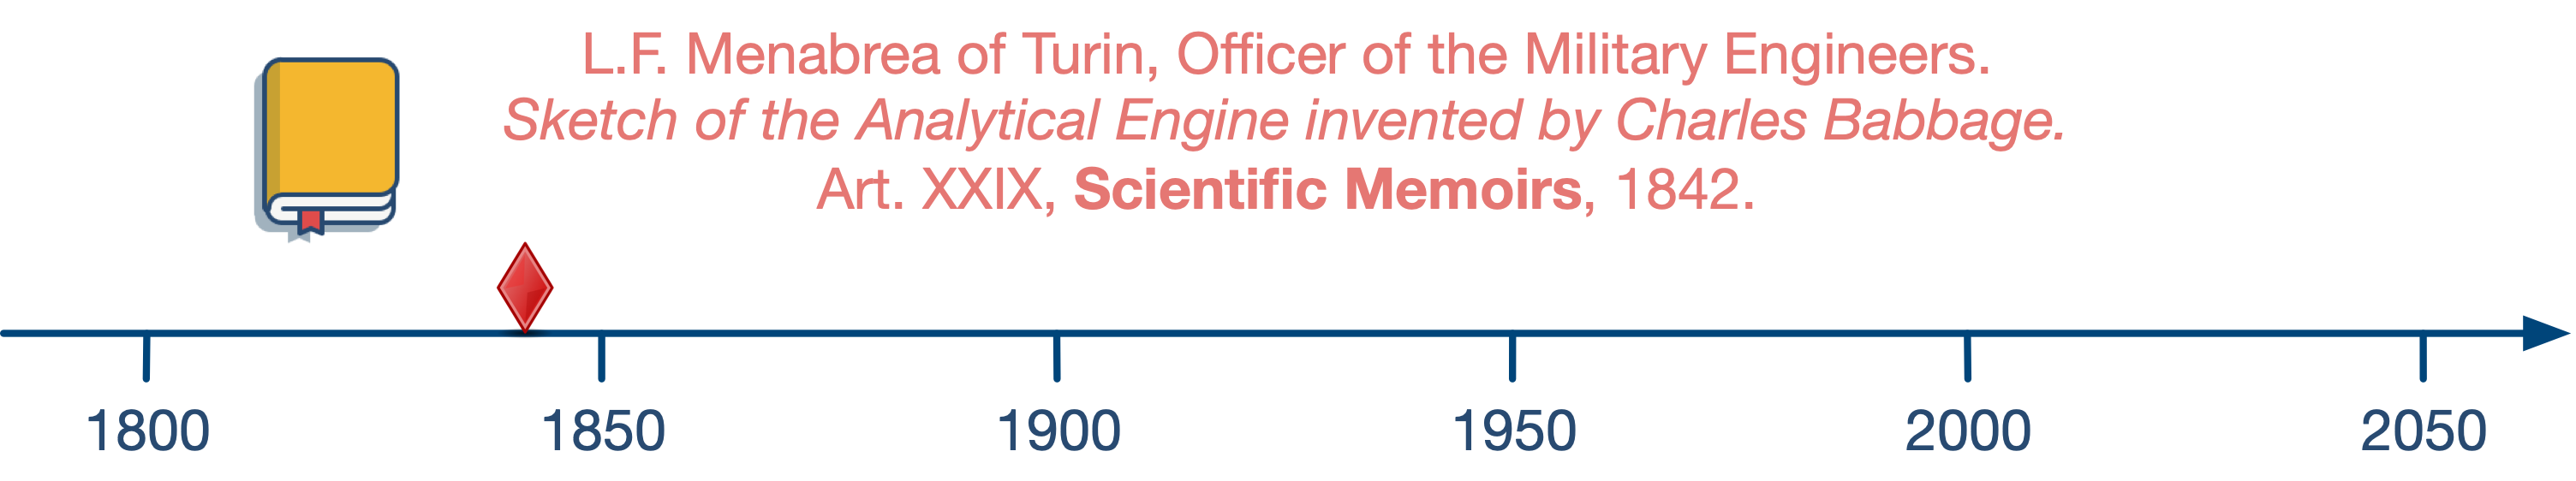
\includegraphics[width=\textwidth]{img/AI-timeline-1842-alt.png}
                \end{figure}
            \end{minipage}
            \\\vspace*{.3cm}
	    	\begin{minipage}[t]{\textwidth}
				\begin{minipage}[t]{0.6\textwidth}
	    			\begin{itemize}[leftmargin=10pt,align=right]
						\onslide<2->\item[\alert{\faHandORight}] Mente visionaria dietro la \alert{macchina analitica di Babbage}
						\onslide<3->\item[\alert{\faHandORight}] Definì per prima il concetto di \alert{ricorsione algoritmica} nel caso della computazione dei numeri di Bernoulli
						\onslide<4->\item[\alert{\faHandORight}] Contributo dimostrato solo un secolo dopo (Harvard Mark I ideato da Howard Aiken e finanziato da IBM nel 1944)
						\onslide<5->\item[\alert{\faHandORight}] Macchina di calcolo che si potesse programmare e riprogrammare per eseguire diverse funzioni (\alert{macchina universale})
					\end{itemize}
            	\end{minipage}
            	%
				\onslide<1->
            	\begin{minipage}[t]{0.4\textwidth}
                	\centering
                	\begin{figure}[ht]
                    	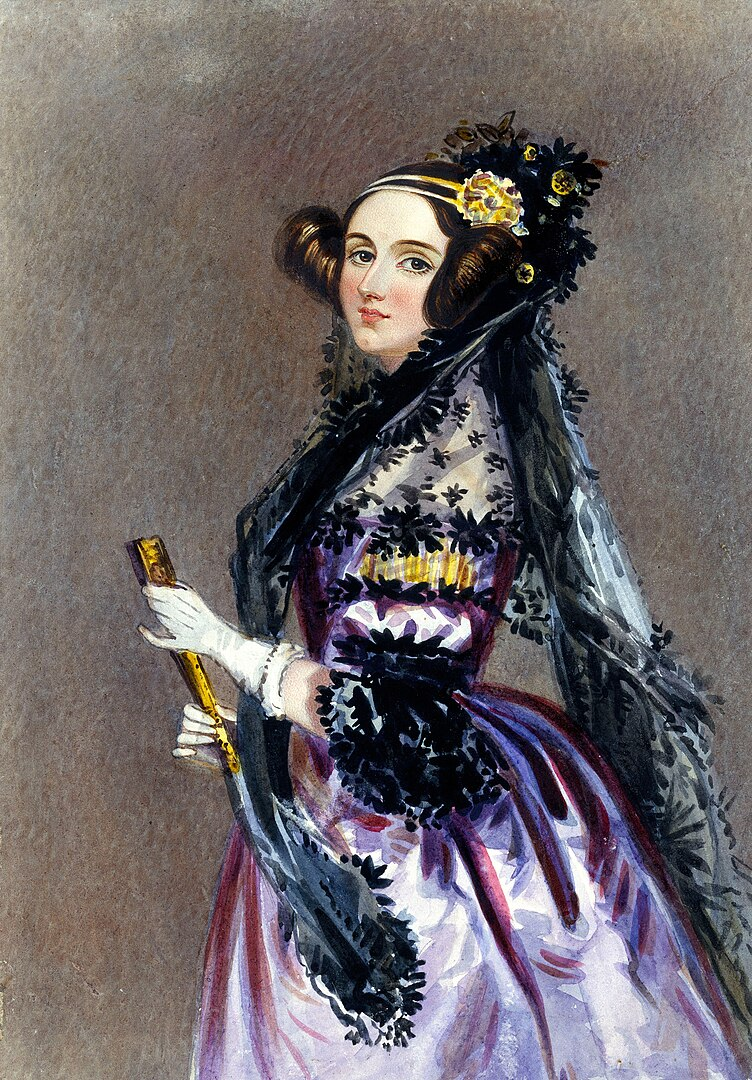
\includegraphics[width=.6\textwidth]{752px-Ada_Lovelace_portrait.jpg}
                    	{\tiny\\Augusta Ada Byron Lovelace\\\textcopyright Wikimedia Creative Commons}
                	\end{figure}
            	\end{minipage}
	    	\end{minipage}
	}
\end{frame}
%
\begin{frame}[t] \frametitle{Nascita della AI}
	{\scriptsize
		\onslide<1->
            \framesubtitle{Dalla macchina al \textit{test} di Turing}
            \vspace*{-.5cm}
            \begin{minipage}[t]{\textwidth}
             	\begin{figure}[ht]
                    \centering
                    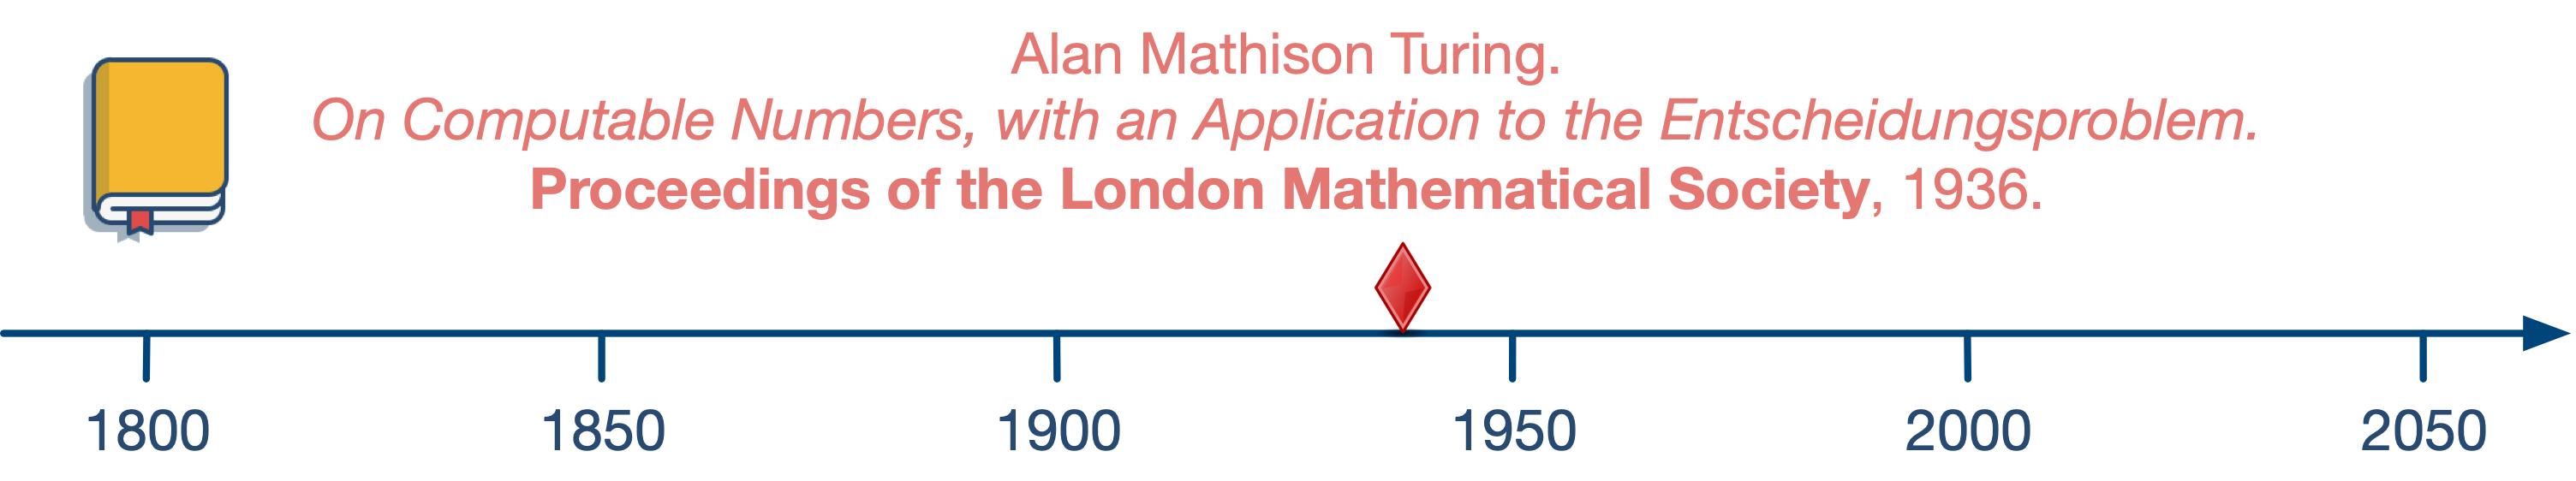
\includegraphics[width=\textwidth]{img/AI-timeline-1936-alt.png}
                \end{figure}
            \end{minipage}
            \\\vspace*{.3cm}
	    	\begin{minipage}[t]{\textwidth}
				\begin{minipage}[t]{0.6\textwidth}
	    			\begin{itemize}[leftmargin=10pt,align=right]
						\onslide<2->\item[\alert{\faHandORight}] Modello di calcolo astratto in grado di eseguire sequenze di istruzioni (\alert{algoritmi}) attraverso lettura e scrittura su nastro e regole (simulazione del processo di calcolo umano)
						\onslide<3->\item[\alert{\faHandORight}] Ogni funzione computabile è Turing-computabile
                    	\onslide<4->\begin{itemize}[leftmargin=10pt,align=right]
							\item[\alert{\faHandORight}] Tutto ciò che una macchina di calcolo reale può computare è calcolabile da una macchina di Turing
							\item[\alert{\faHandORight}] \textit{Standard} per definire la complessità di un algoritmo, la decidibilità o meno di un problema da risolvere
						\end{itemize}
                    	\onslide<5->\item[\alert{\faHandORight}] Ultimo \alert{\textbf{no}} al \alert{problema della decidibilità} di Hilbert (1928)
						\begin{itemize}[leftmargin=10pt,align=right]
							\item[\alert{\faHandORight}] \textit{Esiste una procedura meccanica in grado di decidere in tempo finito se, nell'ambito di una teoria matematica, una data affermazione sia vera o falsa?}
						\end{itemize}
					\end{itemize}
            	\end{minipage}
				%
				\onslide<1->
            	\begin{minipage}[t]{0.4\textwidth}
                	\centering
                	\begin{figure}[ht]
						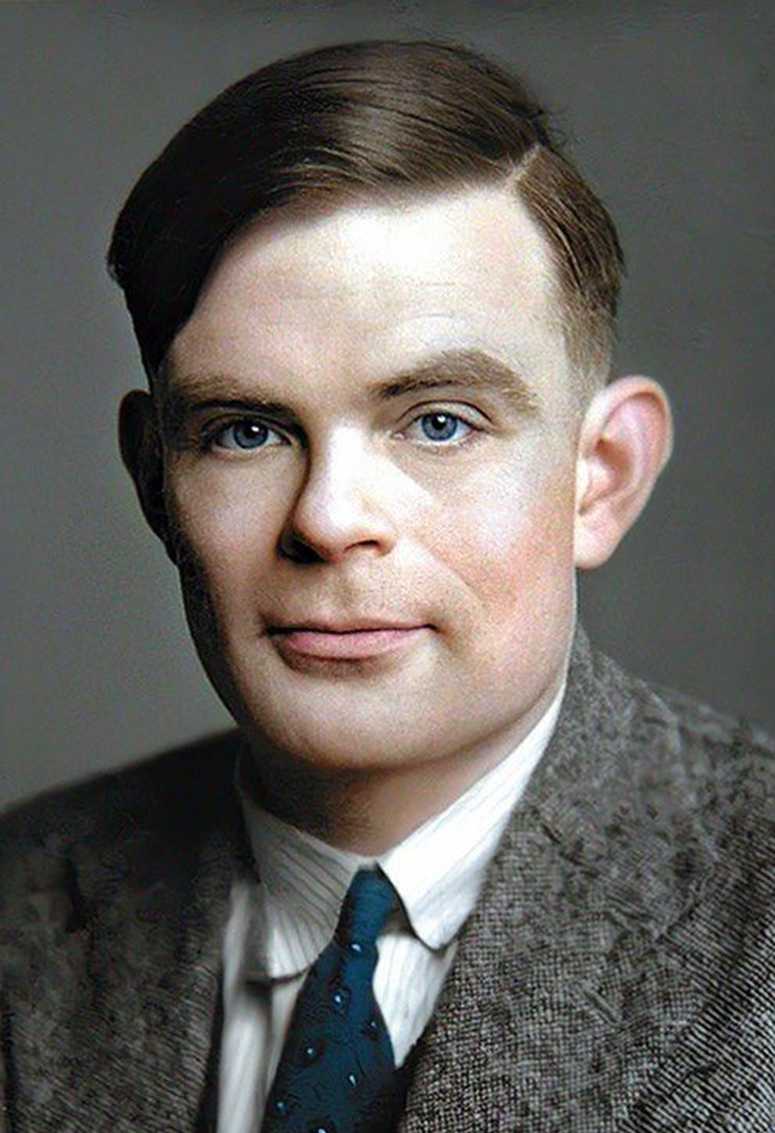
\includegraphics[width=.6\textwidth]{img/alan-turing-color.png}
						{\tiny\\Alan Mathison Turing\\\textcopyright Elcorreo.com}
                	\end{figure}
            	\end{minipage}
	    	\end{minipage}
	}
\end{frame}
%
\begin{frame}[t] \frametitle{Nascita della AI}
    {\scriptsize
    \onslide<1->
        \framesubtitle{Dalla macchina al \textit{test} di Turing}
        \vspace*{-.5cm}
	    \begin{minipage}[t]{\textwidth}
		    \begin{figure}[ht]
			    \centering
			    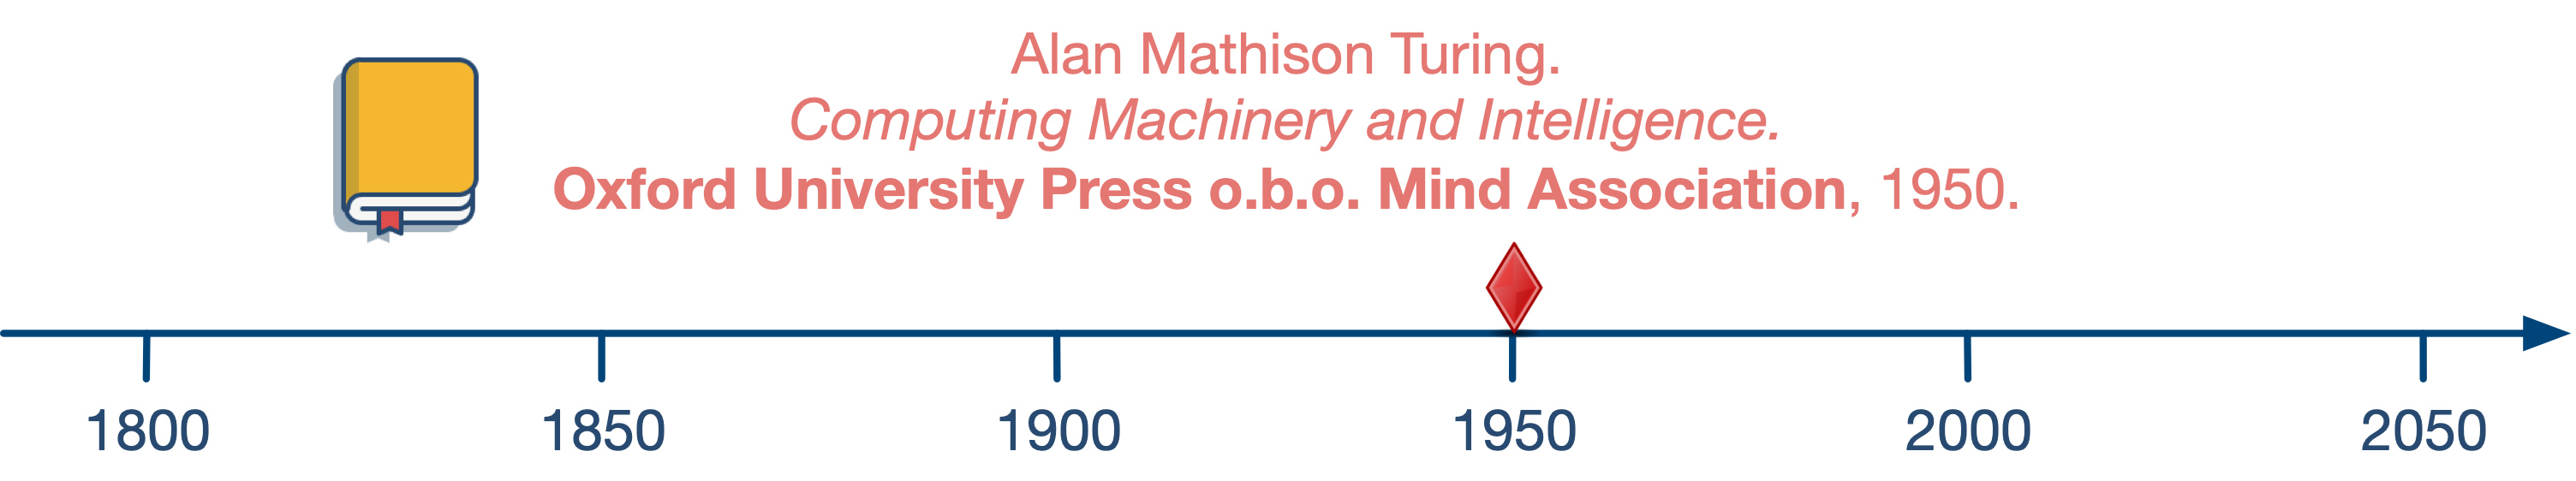
\includegraphics[width=\textwidth]{img/AI-timeline-1950-alt.png}
		    \end{figure}
	    \end{minipage}
	    \\\vspace*{.3cm}
	    \begin{minipage}[t]{\textwidth}
		    \begin{minipage}[t]{0.6\textwidth}
			    \begin{itemize}[leftmargin=10pt,align=right]
				    \onslide<2->\item[\alert{\faHandORight}] Propone il primo esperimento per valutare l'intelligenza di una macchina (\alert{\textit{test} di Turing} o \alert{\textit{Imitation Game}})
				    \onslide<3->\begin{itemize}[leftmargin=10pt,align=right]
						\item[\alert{\faHandORight}] Una macchina e un umano in due stanze separate
						\item[\alert{\faHandORight}] Un arbitro umano pone delle domande a entrambi per definire chi è l'umano dei due
						\item[\alert{\faHandORight}] Se l'arbitro non riesce a determinare la natura degli interlocutori, allora la macchina ha raggiunto un comportamento intelligente
				    \end{itemize}
				    \onslide<4->\item[\alert{\faHandORight}] Impone la comprensione del linguaggio come \alert{condizione sufficiente} dell'intelligenza
			    \end{itemize}
		    \end{minipage}
		    %
		    \onslide<1->
		    \begin{minipage}[t]{0.4\textwidth}
			    \centering
			    \begin{figure}[ht]
				    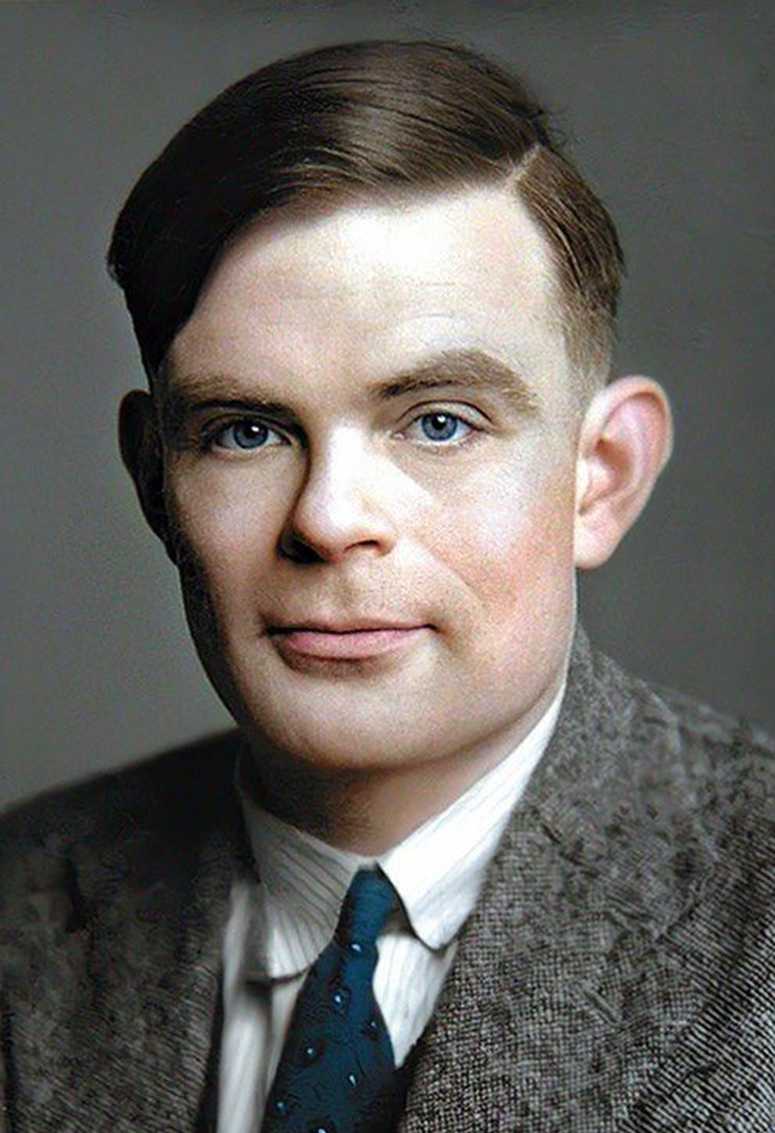
\includegraphics[width=.6\textwidth]{img/alan-turing-color.png}
				    {\tiny\\Alan Mathison Turing\\\textcopyright Elcorreo.com}
			    \end{figure}
		    \end{minipage}
	    \end{minipage}
    }
\end{frame}
%
\begin{frame}[t] \frametitle{Nascita della AI}
{\scriptsize
	\onslide<1->
		\framesubtitle{\textit{Habemus} AI!}
		\vspace*{-.5cm}
		\begin{minipage}[t]{\textwidth}
			\begin{figure}[ht]
				\centering
				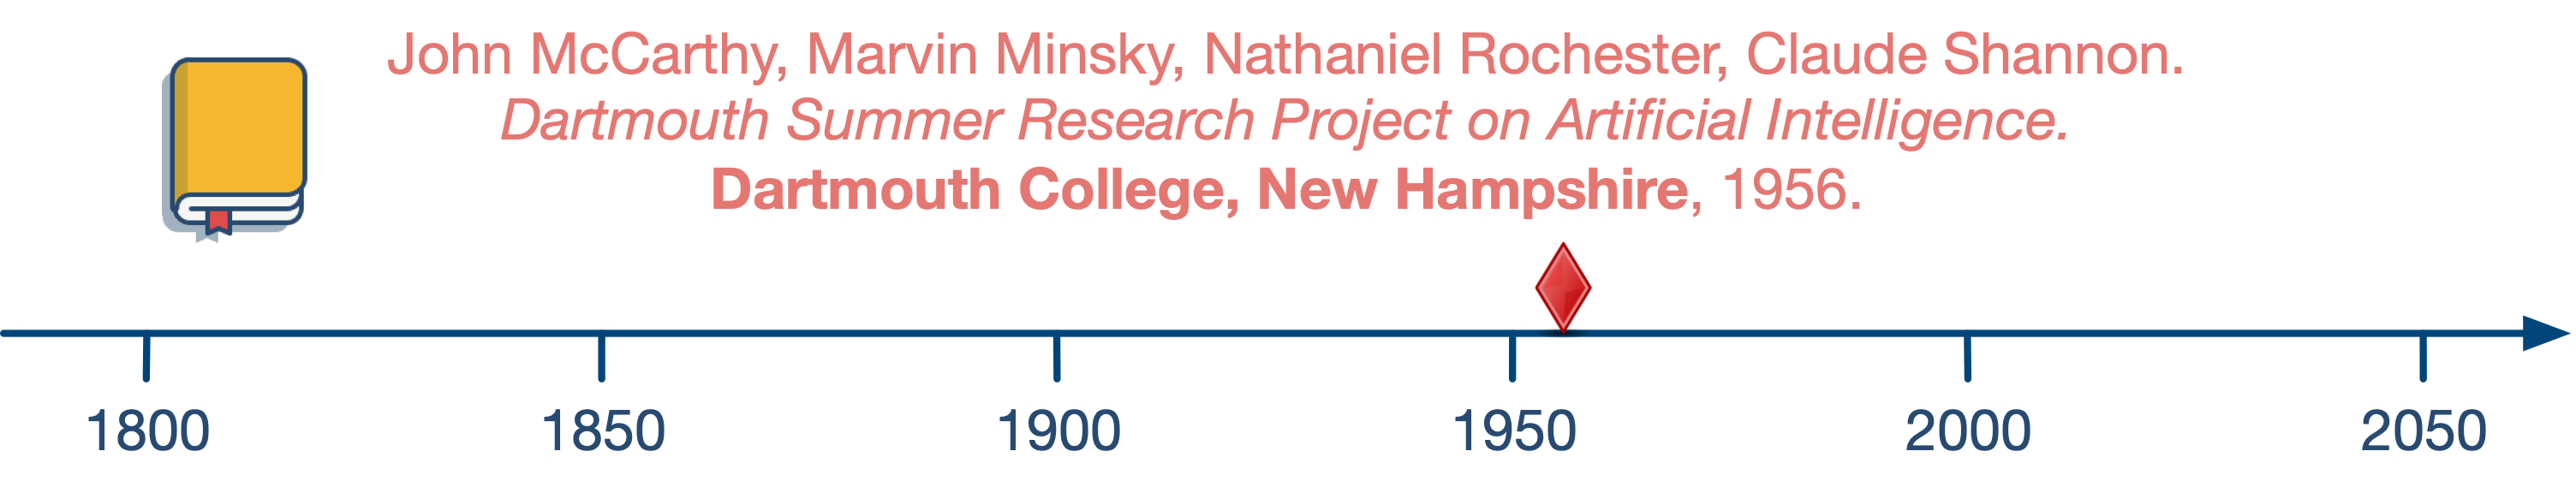
\includegraphics[width=\textwidth]{img/AI-timeline-1956-2-alt.png}
			\end{figure}
		\end{minipage}
	\onslide<1->
    \\\vspace*{.3cm}
	\begin{minipage}[t]{\textwidth}
		\begin{minipage}[t]{0.24\textwidth}
			\centering
			\begin{figure}[ht]
				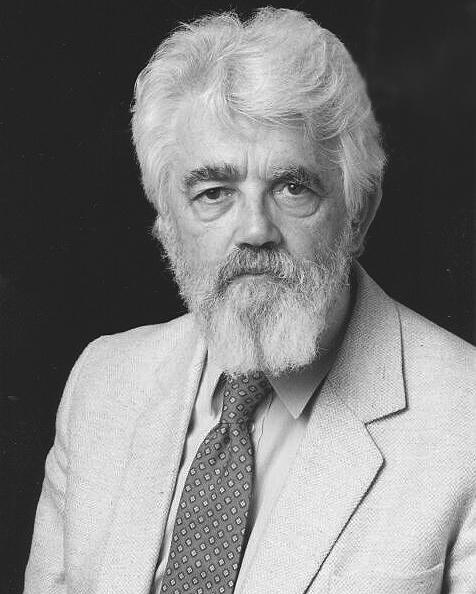
\includegraphics[width=.73\textwidth]{img/John-McCarthy.jpg}
				{\tiny\\John McCarthy\\\textcopyright Naukas}
			\end{figure}
		\end{minipage}
		\begin{minipage}[t]{0.24\textwidth}
			\centering
			\begin{figure}[ht]
				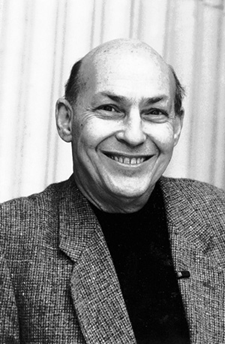
\includegraphics[width=.6\textwidth]{img/Marvin-Misky.png}
				{\tiny\\Marvin Minsky\\\textcopyright Donna Coveny}
			\end{figure}
		\end{minipage}
		\begin{minipage}[t]{0.24\textwidth}
			\centering
			\begin{figure}[ht]
				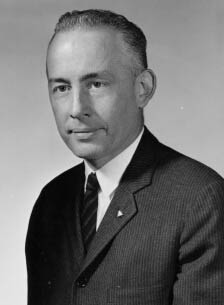
\includegraphics[width=.68\textwidth]{img/Nathaniel-Rochester.jpeg}
				{\tiny\\Nathaniel Rochester\\\textcopyright dmodha}
			\end{figure}
		\end{minipage}
		\begin{minipage}[t]{0.24\textwidth}
			\centering
			\begin{figure}[ht]
				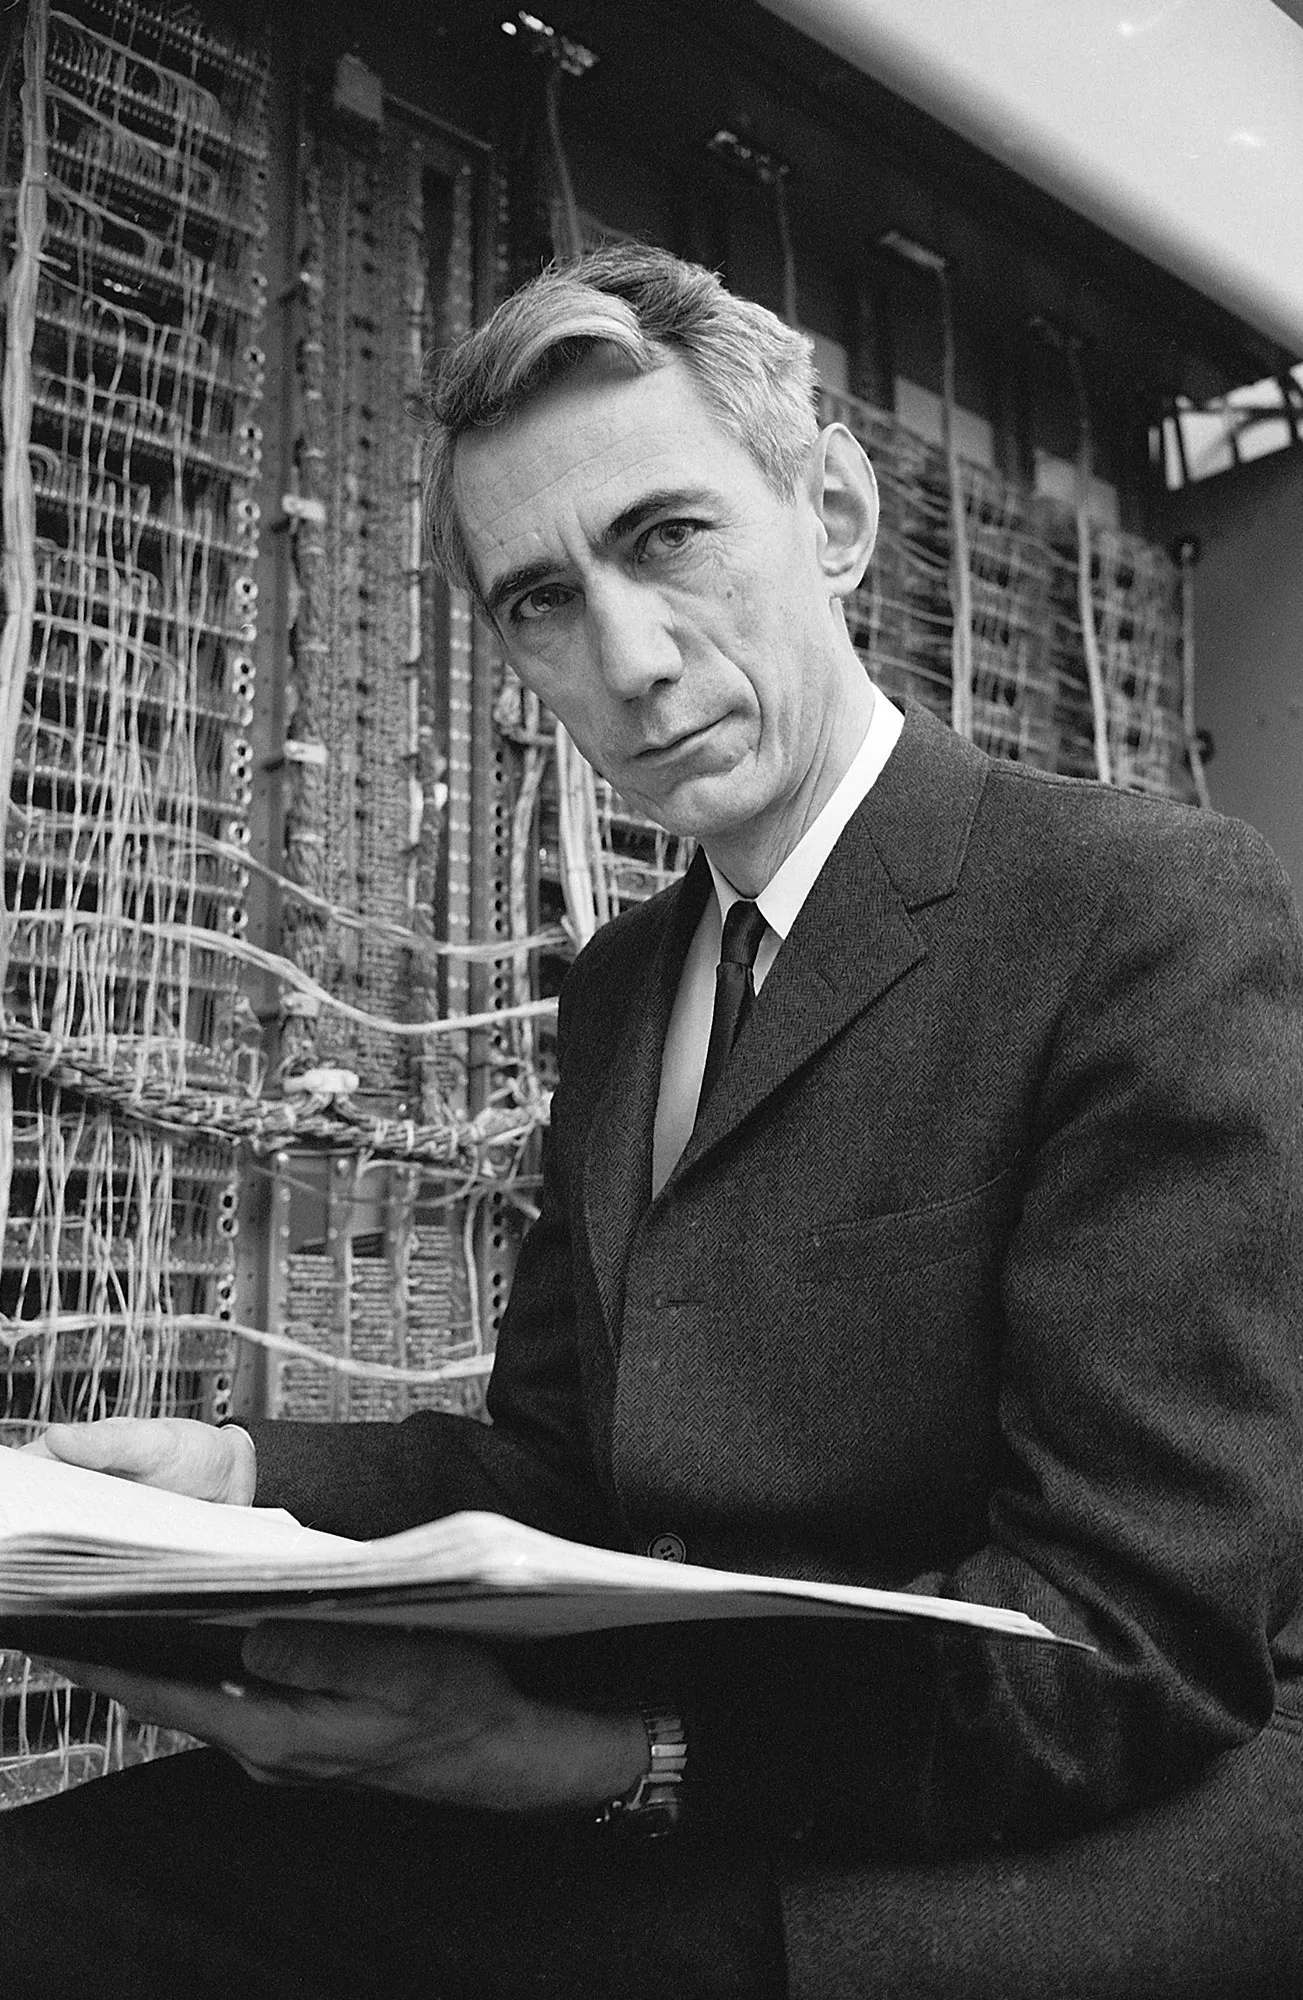
\includegraphics[width=.6\textwidth]{img/Roberts-Claude-Shannon.png}
				{\tiny\\Claude Shannon\\\textcopyright Alfred Eisenstaedt}
			\end{figure}
		\end{minipage}
	\end{minipage}
    \begin{itemize}[leftmargin=10pt,align=right]
		\onslide<2->\item[\alert{\faHandORight}] Coniato ufficialmente il termine \alert{Intelligenza Artificiale}
		\onslide<3->\item[\alert{\faHandORight}] Marca fino al 1974 la \alert{prima estate della AI}
	\end{itemize}
}
\end{frame}
%
\begin{frame}[t] \frametitle{Cronistoria della AI}
	\only<1>{\framesubtitle{1950-1975}}
	\only<2>{\framesubtitle{1975-2000}}
	\vspace*{-.5cm}
	\only<1>{
    	\begin{figure}[ht]
        	\centering
        	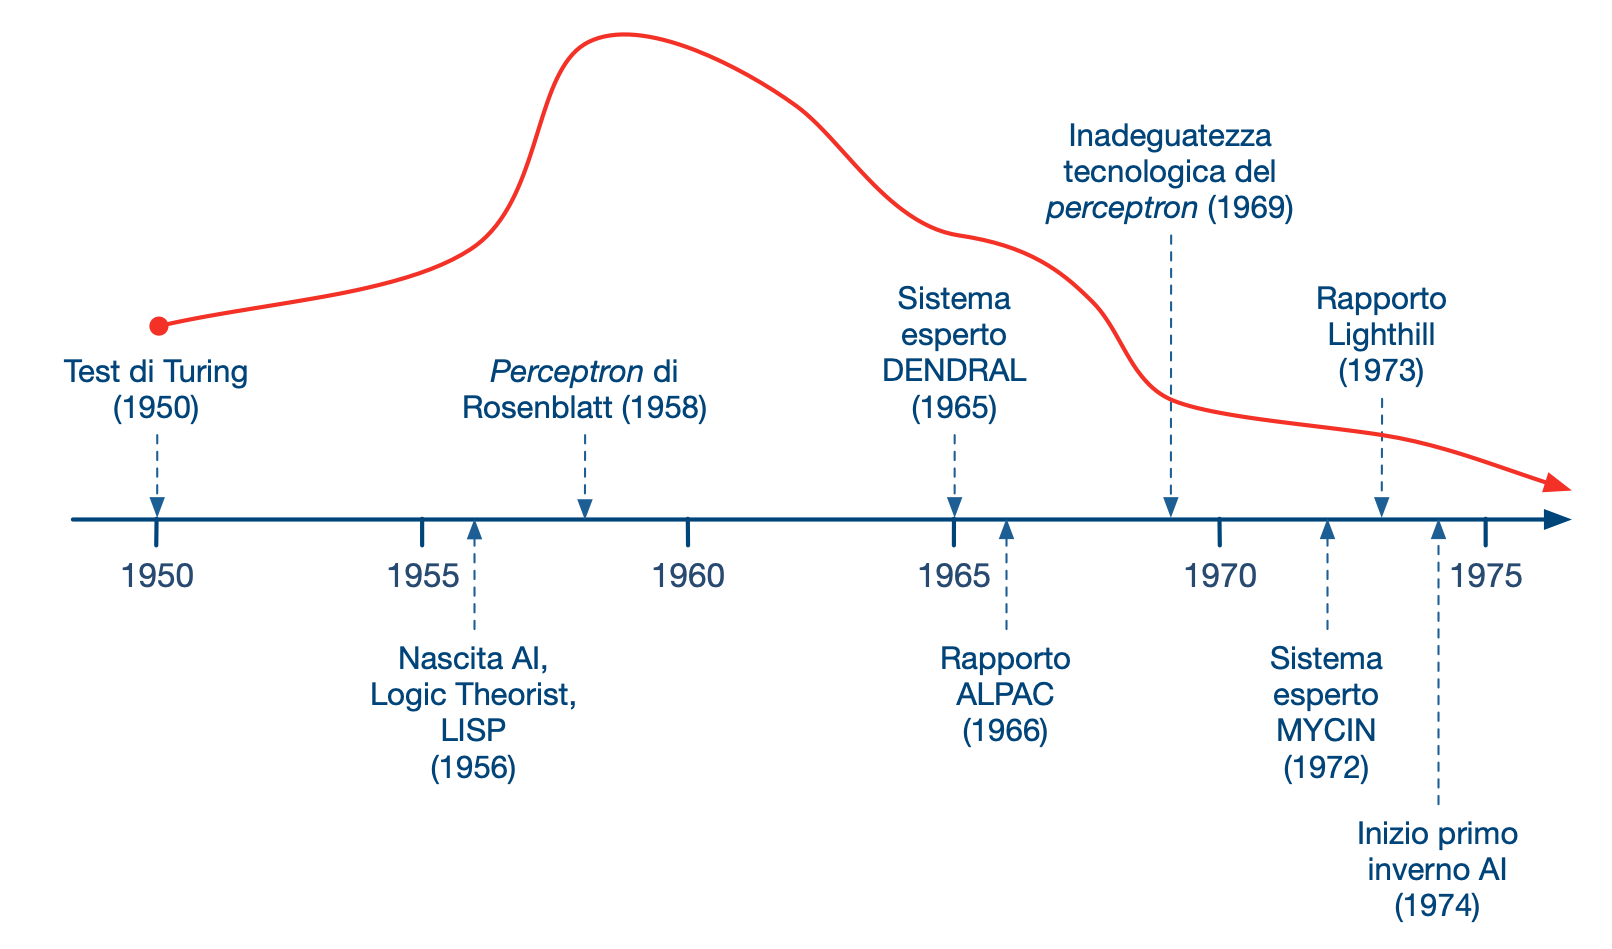
\includegraphics[width=\textwidth]{img/AI-rollercoaster-1.png}
    	\end{figure}
	}
	\only<2>{
    	\begin{figure}[ht]
        	\centering
        	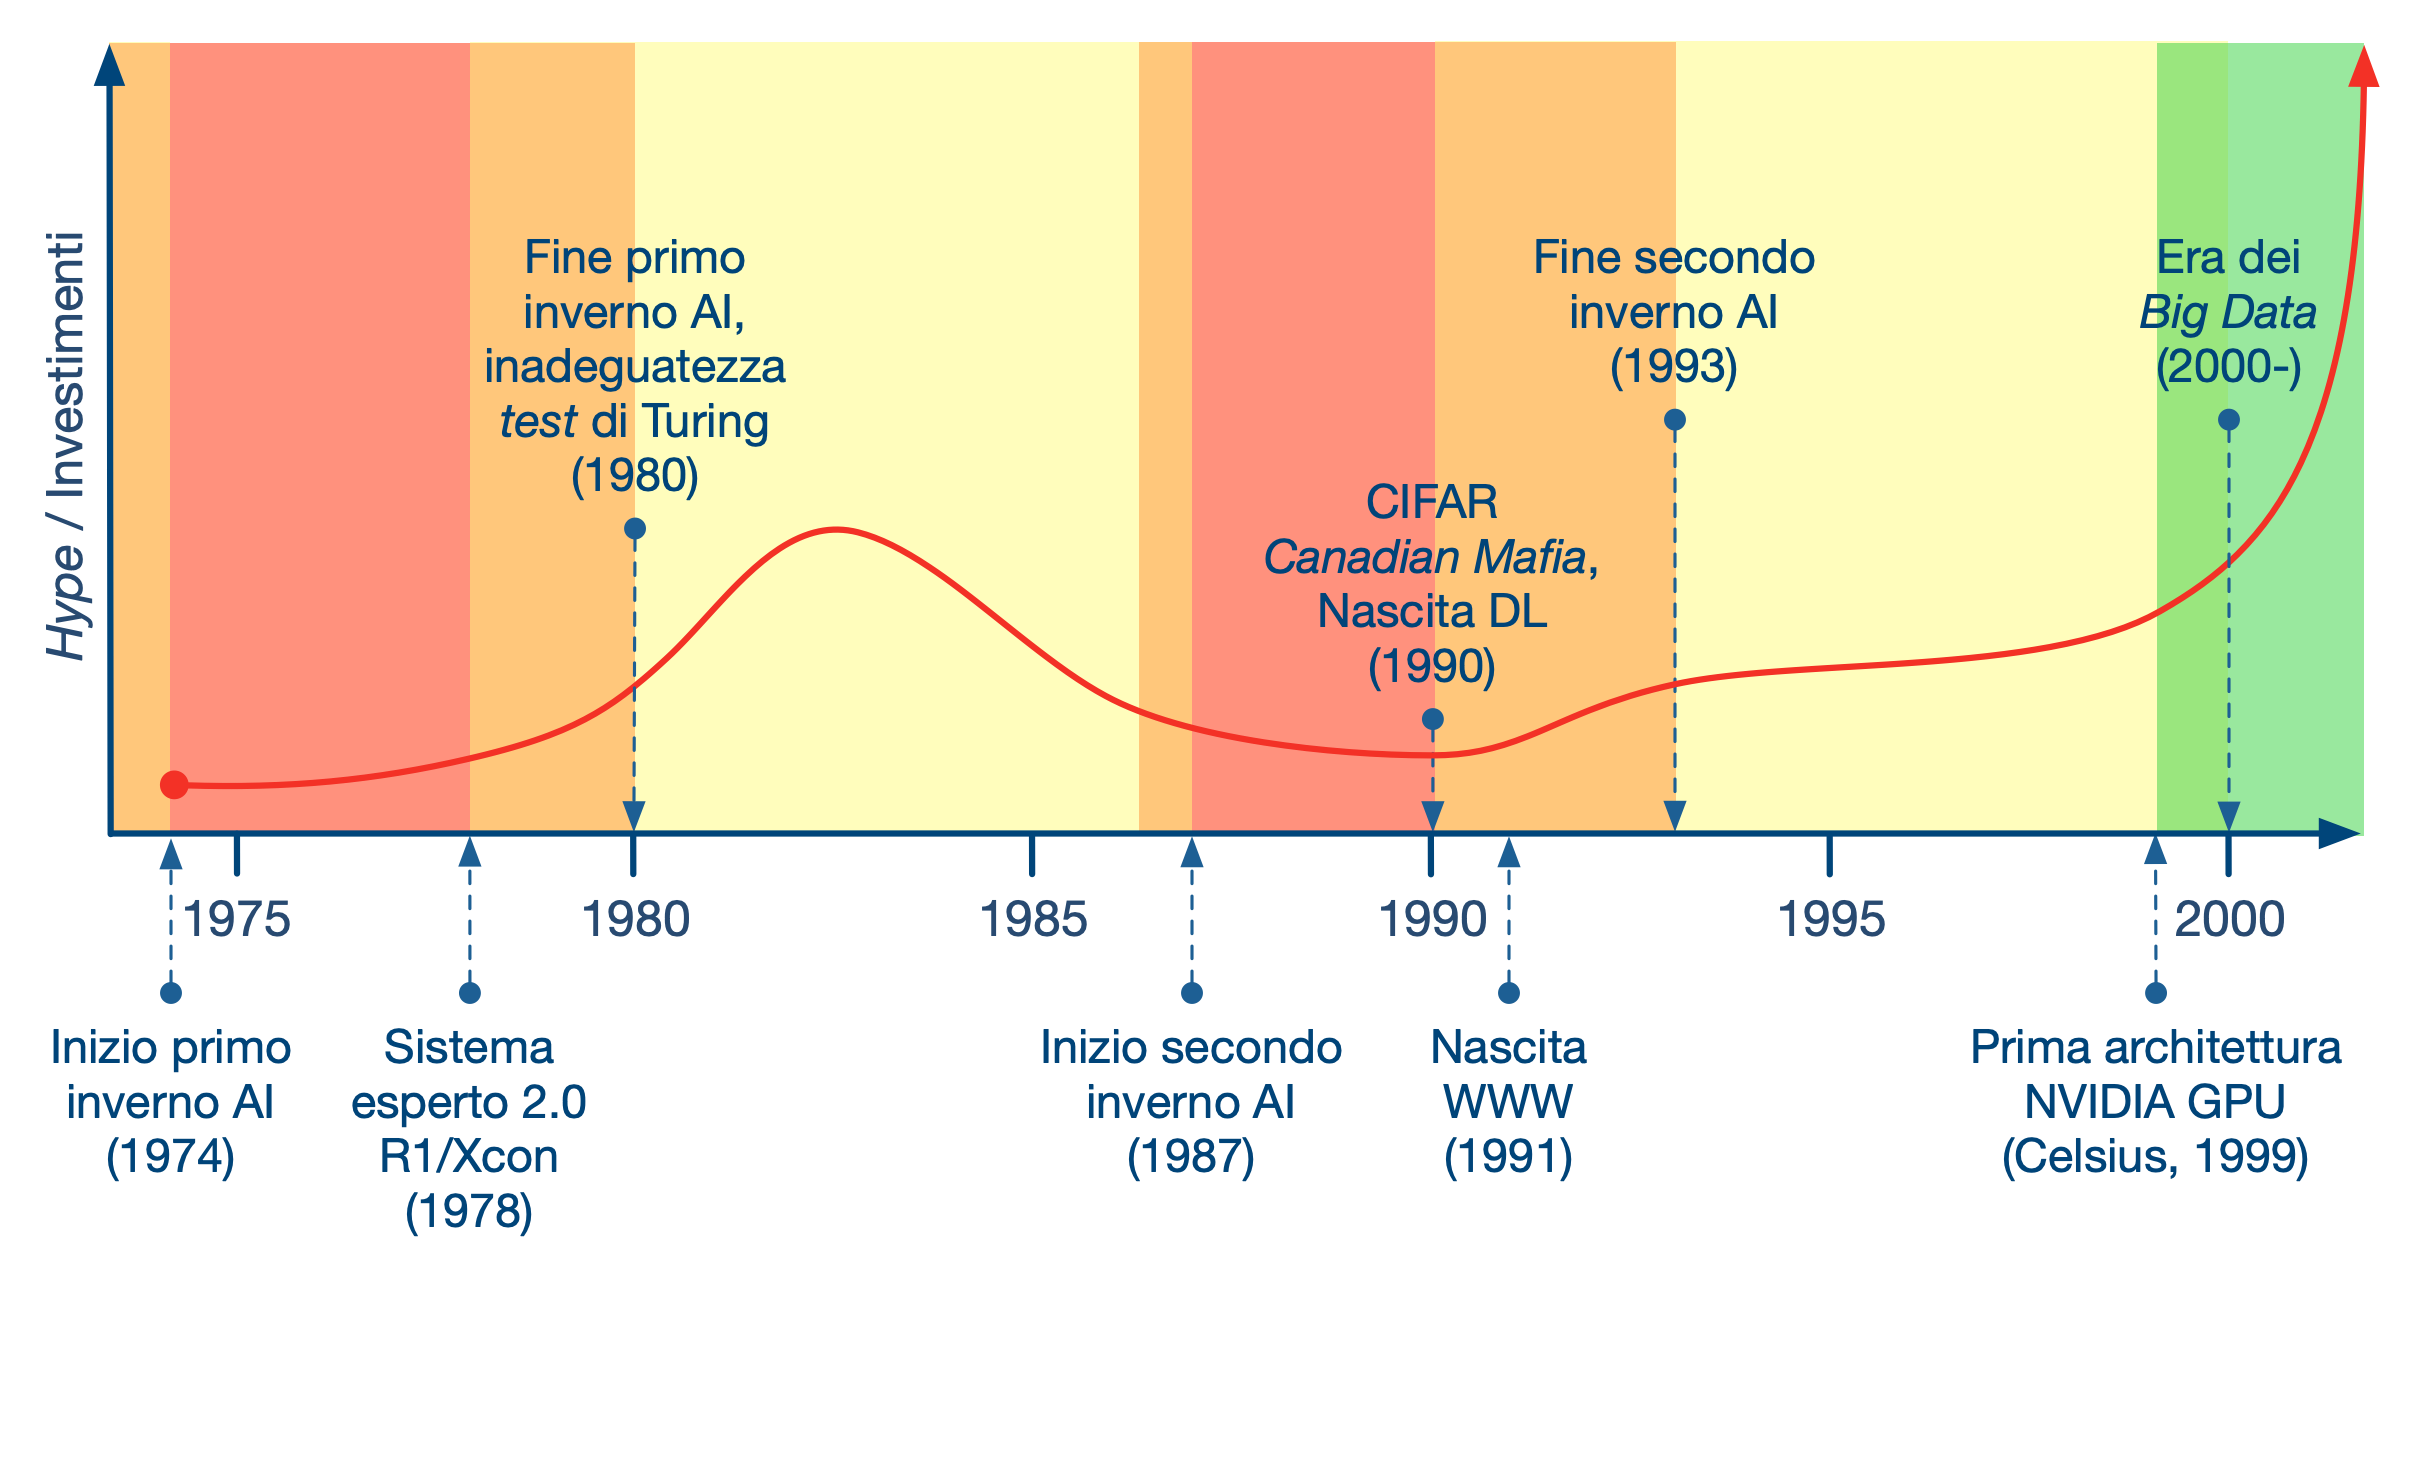
\includegraphics[width=\textwidth]{img/AI-rollercoaster-2.png}
    	\end{figure}
	}
	\begin{flushright}
    	\vspace*{-10pt}
        {\tiny\textcopyright Simone Scannapieco. \textit{I valori delle ordinate sono puramente indicativi.}}
	\end{flushright}
\end{frame}
%
\begin{frame}[t] \frametitle{Intelligenza Artificiale}
{\scriptsize
	\onslide<1->
		\framesubtitle{Secondo il creatore della AI}
		\vspace*{.3cm}
		\begin{minipage}[t]{\textwidth}
			\begin{minipage}[t]{0.45\textwidth}
				\centering
				\begin{figure}[ht]
					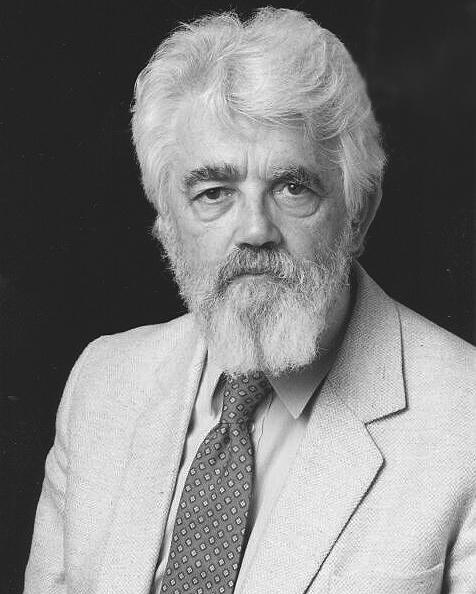
\includegraphics[width=.73\textwidth]{img/John-McCarthy.jpg}
					{\tiny\\\textcopyright Naukas}
				\end{figure}
			\end{minipage}
		    \begin{minipage}[t]{0.5\textwidth}
				\renewcommand{\epigraphsize}{\small}
				\setlength{\afterepigraphskip}{0pt}
				\setlength{\beforeepigraphskip}{5pt}
				\setlength{\epigraphwidth}{\textwidth}
				\epigraph{
					\textit{\alert{D:} Cosa è l'Intelligenza Artificiale?\\
					\alert{R:} E' la scienza e l'ingegneria di creare macchine intelligenti, in particolare programmi informatici intelligenti. È correlata al compito simile di utilizzare i computer per comprendere l'intelligenza umana, ma l'intelligenza artificiale non deve limitarsi a metodi che siano osservabili biologicamente.}}{John McCarthy, \textbf{Stanford Uni, 2007}\\Traduzione: \textcopyright ChatGPT}
			\end{minipage}
		\end{minipage}
}
	\onslide<2->
	\begin{itemize}[leftmargin=10pt,align=right]
		\item[\alert{\faHandORight}] Sistema di AI è un termine estremamente inflazionato\ldots 
		\onslide<3->\item[\alert{\faHandORight}] \ldots anche per sistemi che AI non sono affatto
	\end{itemize}
\end{frame}
%
\begin{frame}[t] \frametitle{NON Intelligenza Artificiale}
	\vspace*{-.5cm}
	\begin{center}
		\begin{minipage}[t]{0.6\textwidth}
			\centering
			\begin{figure}[ht]
				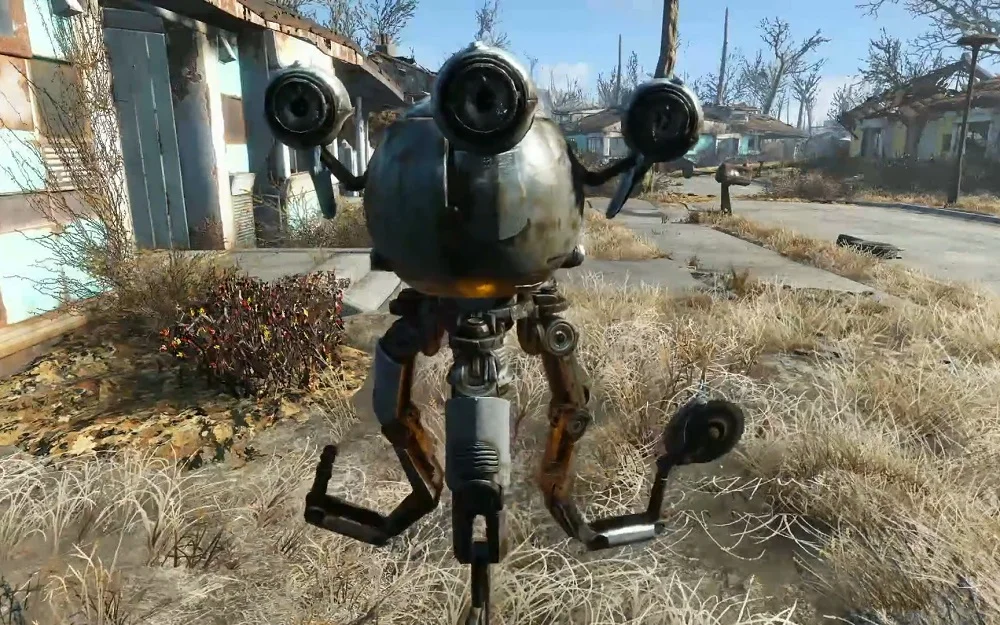
\includegraphics[width=\textwidth]{img/codsworth.png}
			\end{figure}
		\end{minipage}
		\begin{minipage}[t]{.6\textwidth}
			\renewcommand{\epigraphsize}{\tiny}
			\setlength{\afterepigraphskip}{0pt}
			\setlength{\beforeepigraphskip}{5pt}
			\setlength{\epigraphwidth}{\textwidth}
			\epigraph{\textit{Questo significa che sei, ehm\ldots in ritardo di due secoli per cena! Forse potrei prepararti uno spuntino? Devi essere affamato!}}{Codsworth all'Unico Sopravissuto, \textbf{Fallout 4, 2015}\\\textcopyright Nukapedia: The Fallout Wiki}
		\end{minipage}
	\end{center}
	\onslide<2->
	\begin{itemize}[leftmargin=10pt,align=right]
		\item[\alert{\faHandORight}] \alert{\textit{Non-Playable Characters}} (NPC) dei \textit{videogame} 
		\onslide<3->\item[\alert{\faHandORight}] Sistemi di regole \textit{if-then-else}, \alert{non} AI
	\end{itemize}
\end{frame}